\chapter{Estrutura e funcionamento\label{cap:detalhamento-projeto}}

    \section{Processo de instalação\label{sec:processo-instalacao}}
        O \emph{Framework Lothus\{PHP\}} permite ao desenvolvedor a possibilidade de escolha entre dois níves de aplicação. O primeiro nível permite a instalação do \emph{Framework} da forma mais simples, instalando utilitário focados em um desenvolvimento direcionado ao backend do projeto, integrando facilidade a troca de informações com o banco de dados, desenvolvimento através do MVC, URLs amigáves e sistemas de templates.

        Essa instalação é feita através do repositório remoto \emph{Github}, que se encontra no seguinte endereço online:

        \emph{https://github.com/guilouro/Lothus-PHP}

        O Github permite duas formas de download de um projeto: fazendo o downloand de um arquivo comprimido em .zip diretamente do site ou utilizando um sistema de versionamento de arquivos para fazer o clone do mesmo. Neste projetos iremos usar o \emph{Git} como sistema de versionamento. Para fazer o clone utilizando o git executamos a seguinte linha de comando no terminal Unix ou cmd Windows:

        \textbf{\$ git clone https://github.com/guilouro/Lothus-PHP.git}

        Ao executar essa linha de comando, uma nova pasta será criada com o nome de Lothus-PHP. Dentro desta nova pasta estará todo o projeto para iniciar o desenvolvimento utilizando o \emph{Framework Lothus\{PHP\}}. O próximo capítulo será responsável pela apresentação das pastas existentes dentro do projeto.



    \section{Estrutura de pastas e arquivos\label{sec:estrutura-pastas}}
        Neste capítulo será apresentado a estrutura de pastas do \emph{Framework Lothus\{PHP\}} juntamente com o processo de criação e funcionamento de cada etapa.

        Ao clonar o projeto utilizando o git, como visto no capítulo anterior, será gerada uma estrutura de pastas dentro da pasta Lothus-PHP.

        \begin{figure}[!htb]
            \centering
            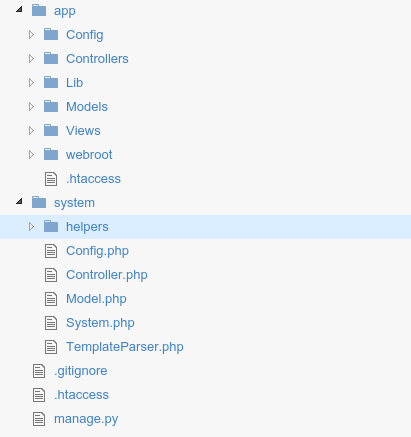
\includegraphics[scale=0.8]{pastas.jpg}
            \caption{\small Estrutura do projeto}
            \label{cap:sass}
        \end{figure}

        Neste primeiro momento já ocorre uma pequena divisão do projeto onde a pasta \emph{app} é responsável por gerenciar a aplicação e a pasta \emph{system} responsável pelo \emph{core}, ou seja, gerenciamento interno do framework. Em sua raiz existe, além dessas duas pastas, três importantes arquivos para o projeto, que são:

        \begin{itemize}
            \item \textbf{.gitignore}: Um arquivo que faz parte da configuração do git e é responsável por guardar, linha por linha, todos os arquivos ou pastas serão ignorados pelo git no momento de fazer o versionamento do projeto. Isso evita o acumulo de arquivos desnecessários, que são gerados automaticamente, no pacote de instalação do Framework.

            \item \textbf{.htaccess}: Arquivo que é lido antes do index.php e tem a responsabilidade de criar a rota inicial do projeto, fazendo o direcionamento para o arquivo correto na inicialização do sistema.

            \begin{figure}[!htb]
                \centering
                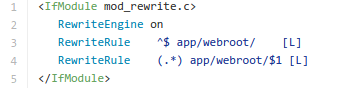
\includegraphics[scale=0.8]{htaccess1.jpg}
                \caption{\small Estrutura do htaccess na raiz do projeto}
                \label{cap:sass}
            \end{figure}

            \item \textbf{manage.py}: Trata-se de um script de linha de comando capaz de gerar novos arquivos baseados na arquitetura de funcionamento do \emph{Framework}. A imagem abaixo ilustra o uso básico da ferramenta.

            \begin{figure}[!htb]
                \centering
                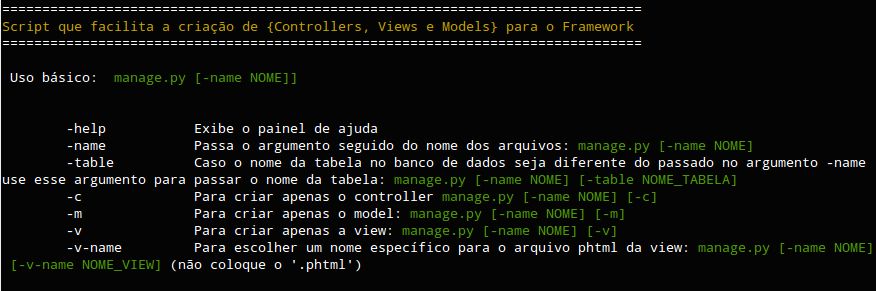
\includegraphics[scale=0.5]{manage.jpg}
                \caption{\small Regras para uso básico do manage.py}
                \label{cap:sass}
            \end{figure}


        \end{itemize}

    \section{System\label{sec:system-core}}

        A pasta \emph{system} é o motor do \emph{Framework}, nela estão todas as classes responsáveis pelas regras de funcionamento dos projetos, tanto nas requisições HTTP, passando por padronização de Controllers, Views e chegando até o relacionamento com o banco de dados. Todas essas funcionalidades estão divididas entre classes e arquivos alocados dentro de \emph{system}.

            \begin{figure}[!htb]
                \centering
                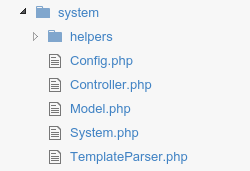
\includegraphics[scale=1]{system-path.jpg}
                \caption{\small Estrutura interna da pasta system}
                \label{cap:sass}
            \end{figure}




\begin{lstlisting}
private function setUrl() {
    $this->_url = (isset($_GET['url']) ? $_GET['url']  : $this->_Index . "/index_action" );
}
\end{lstlisting}


        \subsection{Helpers\label{sub:system-helper}}

        \subsection{Config\label{sub:system-config}}

        \subsection{Controller\label{sub:system-controller}}

        \subsection{Model\label{sub:system-model}}

        \subsection{System\label{sub:system-system}}

        \subsection{Template\label{sub:system-template}}





    \section{Divisão Backend - frontend\label{sec:back-front}}


        \subsection{Comandos do Grunt\label{sub:comandos-grunt}}

    \section{System\label{sec:estrutura-pastas}}

    \section{Model\label{sec:estrutura-pastas}}

    \section{View\label{sec:estrutura-pastas}}

    \section{View\label{sec:estrutura-pastas}}

    \section{Template\label{sec:estrutura-pastas}}
